



\chapter{Jets in Proton-Proton Collisions}%\label{ch1:intro}



A jet is a collimated grouping of hadrons usually associated with the LO production of a parton, quark or gluon. In this case the quark (gluon) could be initiated by the hard scatter of 2 constituent partons from protons or be the decay product of another particle that was produced in the hard scatter, such as a W boson, which can then decay to 2 quarks each forming a jet. The initial parton radiates other quarks and gluons, called the "Parton Shower" and all color charged particles fragment into hadrons, mainly pions and kaons,  before reaching the detector as mentioned in ~\ref{chap:MCGenReco}.

Studies of jets at LHC are complicated by experimental complexities such as "underlying event", other partons from the same proton interacting and depositing energy in the same region of the detector. "Pileup" is also increasingly relevant, like "underlying event" but initiated from other proton interactions from this or a previous bunch, since the LHC crosses bunches with $~10^{11}$ protons every 25 nanoseconds.



Any measurement is limited by the resolution of the measurement device and any detector effect. In this thesis the results are disentangled from the reconstructed data by "unfolding" the reconstructed distributions back to generator level.

While jets are often used as simple proxies for the quark or gluon from which they originated, the structure of the radiation pattern of the hard scatter is encoded within the jet's constituent particles~\cite{Asquith:2018igt}. Jet studies are essential for a complete understanding of proton-proton interactions since the majority of interesting physics signatures contain a color charged parton in the final state. This chapter covers the basics of jet physics at LHC, from the algorithms used for clustering the constituent particles in experimental data to the language and calculations of the theory.

% cite https://arxiv.org/pdf/1901.10342.pdf simones book



\section{Jet Clustering Algorithms}\label{secSM:ch1}

At LO, a jet represents a quark [gluon], however realistically that is not a well defined concept and a more precise definition is useful. This thesis adopts the definition presented at the Les Houghes conference in 2015 :\newline

"A phase space region (as defined by an unambiguous hadronic fiducial cross section measurement) that yields an enriched sample of quarks [gluons] (as interpreted by some suitable, though fundamentally ambiguous, criterion)"~\cite{Badger:2016bpw}.\newline 

I will discuss one class of "suitable, though fundamentally ambiguous" criteria for defining jets, known as sequential recombination algorithms. These algorithms take pairs of particles and successively combine them into 1 particle, in a way which is intended to reconstruct the successive branchings of partons within the jet as described by perturbative QCD ~\cite{Marzani:2019hun}.
 
% rivello: Broken citation at the paragraph below:
In sequential recombination algorithms a distance metric, $d_{ij}$, is defined between all particle pairs. These pairs are then sequentially combined in order of increasing distance. Three popular algorithms in this class can be described by the equation ~\ref{eq:sequRec}:


\begin{equation}
\begin{array}{l}{d_{i j}=\min \left(p_{t i}^{2 p}, p_{t j}^{2 p}\right) \frac{\Delta R_{i j}^{2}}{R^{2}} \quad \Delta R_{i j}^{2}=\left(y_{i}-y_{j}\right)^{2}+\left(\phi_{i}-\phi_{j}\right)^{2}} \\ {d_{i B}=p_{t i}^{2 p}}\end{array}
\end{equation}\label{eq:sequRec}


Depending on the value chosen for $p$, this equation can produce a variety of clusterings, herein I discuss the 3 popular choices $p = [1, 0, -1]$ referring to them by their names: KT ~\cite{Ellis:1993tq}, Cambridge/Aachen ~\cite{Dokshitzer:1997in} and Anti\kt algorithms ~\cite{Cacciari:2008gp} respectively.

Each algorithm has its own specific use cases and drawbacks. For example, the Anti\kt algorithm produces circular jets of constant area as seen in ~\ref{fig:antikt}. 

\begin{figure}[htb]
\centering
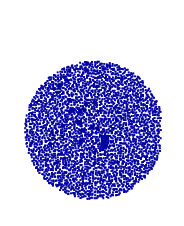
\includegraphics[width=.40\textwidth]{visuals/figs_subjet-plots-antikt.png}
\caption{For jets clustered using the Anti\kt algorithm a circular pattern emerges, making pileup and underlying event subtraction simpler for experimentalists~\cite{Dreyer:2018nbf}.}
\label{fig:antikt}
\end{figure}



This constant area is useful for experimental studies as it allows for simple removal of underlying event energy, which is evenly distributed throughout the jet area ~\cite{Dreyer:2018nbf}. In contrast to the other 2 algorithms described, the C/A algorithm does not contain any momentum weighting, this leads to jets which are not circular, depicted in ~\ref{fig:cashape}, and instead follow the radiation pattern of the original jet constituent particles as seen in ~\ref{fig:cashape}. The variation in the way these algorithms cluster the underlying radiation is depicted in ~\ref{fig:algclusterdiffs}. In this thesis we have chosen to recluster the Anti\kt jets with C/A in order to preserve the original radiation pattern.


%##image C/A vs anti-Kt --- visuals/config-antikt-double-lund
\begin{figure}[htb]
\centering
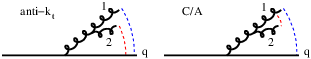
\includegraphics[width=1.0\textwidth]{visuals/config-antikt-double-lund.png}
\caption{Notice that the clustering follows the radiation pattern for C/A while the softer emissions are clustered with the jet axis in the case of Anti\kt ~\cite{Dreyer:2018nbf}.}
\label{fig:algclusterdiffs}
\end{figure}


\begin{figure}[htb]
\centering
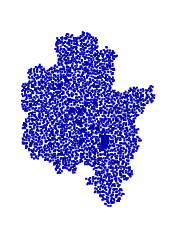
\includegraphics[width=.40\textwidth]{visuals/figs_subjet-plots-CA.png}
\caption{Jets clustered using C/A algorithm are not circular, instead they are shaped like the radiation pattern~\cite{Dreyer:2018nbf}.}
\label{fig:cashape}
\end{figure}


% good section on it here
% http://inspirehep.net/record/1123042/files/fermilab-thesis-2012-12.pdf

%# https://arxiv.org/pdf/1304.1025.pdf
%Sequential recombination algorithm for jet clustering and








%#

%#


\section{Jet Grooming}\label{sec:jetgroom}

Jet grooming is a broad term to describe a number of different algorithms intended to remove some portion of the soft and collinear radiation within a jet. This analysis uses the Soft-Drop (SD) algorithm~\cite{softdrop} which removes soft and collinear radiation in a theoretically controlled manner. The SD procedure is as follows: Begin with an Anti\kt ~\cite{Cacciari:2008gp} clustered jet composed of particle flow candidates, reclustered with Cambridge-Aachen algorithm~\cite{Dokshitzer:1997in} to remove the \pt weighting dependence of the clustering. At this stage we regress through the clustering history, keeping a subjet if it meets of SD criterion and otherwise "dropping" it.

% FIX ME ref particle flow section

SD iteratively declusters a jet $j$ with distance parameter $R$ into two subjets, $j_1$ and $j_2$.
If the softdrop condition

\begin{equation}
  \frac{\min(p_{T1},p_{T2})}{p_{T1}+p_{T2}} > z_{cut} \cdot (\frac{\Delta R_{12}}{R})^\beta
\end{equation}

is met, then the procedure terminates and $j$ is the final state jet. Otherwise, the declustering continues - 
the higher $\pt$ subjet is relabeled as $j$ and the lower $\pt$ ("softer") subjet is dropped, hence the name.
By design, this condition fails for wide-angle soft radiation, which is therefore removed by the soft
drop procedure. The tunable parameters, $\beta$ and $z_{cut}$, control the degree of jet grooming:
$\beta$ tunes the algorithm's sensitivity to wide-angle radiation, while $z_{cut}$ sets the energy scale
of the grooming. In the case of $\beta \rightarrow \infty$, an ungroomed jet is returned. 
In the $\beta = 0$ case, the soft drop procedure is identical to the ``modified mass drop tagger'' (MMDT)
from Ref.~\cite{mmdt}. For $\beta > 0$  soft emissions are removed from the jet while the majority of the collinear emissions remain, as illustrated in ~\ref{fig:softdroplund}. 


\begin{figure}[htb]
\centering
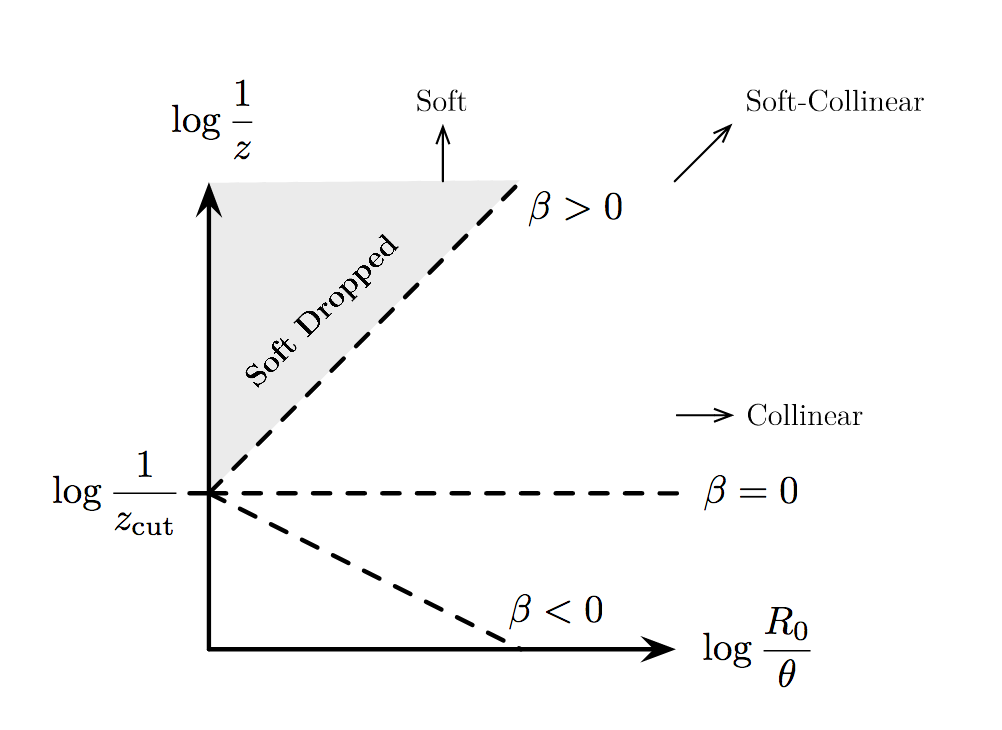
\includegraphics[width=1.0\textwidth]{visuals/softdroplund.png}
\caption{An illustration of the phase space for jet emissions outlining which would be groomed away by the SD procedure ~\cite{softdrop}.}
\label{fig:softdroplund}
\end{figure}
%#

The soft drop algorithm removes soft and wide-angle radiation
from jets in a very theoretically controlled manner, making it suitable to separate
the ``hard'' and ``soft'' parts of the jet. Specifically, the soft drop
algorithm can remove non-global logarithms from correlations of
radiation within and between jets, which are extremely difficult to
compute theoretically~\cite{Dasgupta:2001sh,mmdt,softdrop,Dasgupta:2013via,Dasgupta:2015yua,Larkoski:2015zka}.



%Casimir Meets Poisson: Improved Quark/Gluon Discrimination with Counting Observables
%https://arxiv.org/abs/1704.06266
%soft drop multiplicity







%%%%%%%%%%%%%%%%% Lund Jet Plane



\section{Lund Jet Plane}\label{sec:lundjetplane}



A Lund kinematic Diagram, shown in  ~\ref{fig:introlund}, is an illustration of the kinematics of emissions within a jet in terms of two variables: horizontally, the logarithm of the inverse of the angle of a given emission with respect to the jet axis, and vertically the logarithm of the emission's transverse momentum $k_t$. The line of constant jet mass and the shaded region constitute the part of the phase space in which emissions are vetoed, this leads to a Sudakov form factor~\cite{mmdt}.

The Lund kinematic diagram, or Lund jet plane, is a theoretical representation of the phase space within jets, and has been a useful tool for studying parton showers in the past, and has now been extended to individual jets through repeated Cambridge/Aachen declustering ~\cite{Dreyer:2018nbf}.



\begin{figure}[htb]
\centering
\includegraphics[width=.90\textwidth]{visuals/introlund.png}
\caption{A Lund kinematic Diagram. The line of constant jet mass is shown in red~\cite{mmdt}.  }
\label{fig:introlund}
\end{figure}



\begin{figure}[htb]
\centering
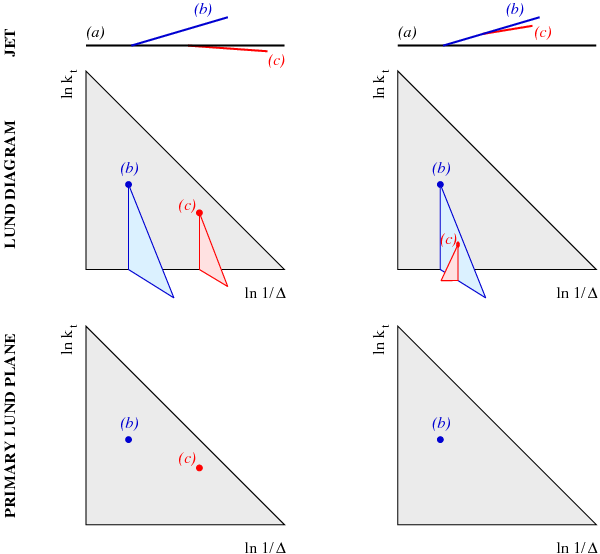
\includegraphics[width=1.0\textwidth]{visuals/figs_lund.png}
\caption{The primary and secondary lund planes for 2 example jets~\cite{Dreyer:2018nbf}.}
\label{fig:lundPrimaryandSecondary}
\end{figure}


The primary Lund plane is shown on the bottom of Figure ~\ref{fig:lundPrimaryandSecondary} ~\cite{Dreyer:2018nbf} where the black particle (a) "initiated" the jet and is described by the grey shaded region and particles (b) and (c) are marked with dots and constitute emissions within the jet. In contrast, the Lund diagram shows the phase space encompassed by each subsequent emission, not just the emission (a).~\cite{Dreyer:2018nbf}
%image 



%%%%%%%%%%%%%%%%% Jet Mass section



\section{Jet Mass}\label{sec:jetmass}


The calculations for the jet mass in perturbative QCD are described in this section. Jet invariant mass is a simple observable, useful for probing QCD, it is defined as:\newline

\begin{equation}
m^{2}=\left(\sum_{i \in \mathrm{jet}} k_{i}\right)^{2}
\end{equation}

the summation includes all particles $i$ clustered into the jet. In the case of this thesis the particles are particle-flow candidates, Section ~\ref{sec:PFReco} contains information on how the events for this thesis were reconstructed.

The plain jet mass is discussed in the first subsection while a later subsection shows how the jet mass distribution is calculated for jets modified by a "grooming" algorithm, in this case soft-drop ~\cite{softdrop} , as are the jets in the groomed measurement presented herein.

This discussion centers on "QCD jets", initiated by a hard parton and evolving via a parton shower but stopping at parton level as perturbation theory is not able to describe the transition to particle level~\cite{Marzani:2019hun}. Event generators employ different hadronization techniques to describe the parton-to-hadron transition, those used in this thesis are discussed in Section ~\ref{secMCGen}.

Within the valid phase space of perturbative QCD on finds that the fixed-order approach to jet mass is inadequate, most noticeably in the boosted regime as each emission contributes a large logarithm~\cite{Marzani:2019hun}. All-order resummation techniques are then exploited to theoretically describe the jet mass observable more accurately than is possible with fixed-order. 



\subsection{Plain Jet Mass }\label{sec:jetmass}


In this section quark jet mass calculations are discussed at LO. It is first useful to define the dimensionless jet mass, $\rho$ , as the plain mass is $\pt$ dependent.


\begin{equation}
\rho=m^{2} /\left(E^{2} R^{2}\right)
\end{equation}



Using the small-angle approximation, $\rho$ is invariant under Lorentz boosts along the jet axis direction, since boosts vary the jet $\pt$ up by some factor (say $\kappa$ ) and scale its opening angle by the inverse factor ($\frac{1}{\kappa}$) while leaving the mass unchanged. Due to this invariance, the analytical results are often simplest when expressed in terms of $\rho$ ~\cite{mmdt}.

Now the integrated jet mass distribution can be defined as :\newline

\begin{equation}
D(\rho)=\int_{\rho}^{1} \frac{d \rho^{\prime}}{\rho^{\prime}} \int_{\rho^{\prime}}^{1} d z p_{g q}(z) \frac{\alpha_{s}\left(z \rho^{\prime} R^{2} p_{t}^{2}\right) C_{F}}{\pi}
\end{equation}


Above the quark-gluon splitting function is $p_{g q}=\frac{1+(1-z)^{2}}{2 z}$. This can be elucidating if we take the fixed coupling approximation to reveal the below relationship.~\cite{mmdt}


\begin{equation}
D(\rho) \simeq \frac{\alpha_{s} C_{F}}{\pi}\left[\frac{1}{2} \ln ^{2} \frac{1}{\rho}-\frac{3}{4} \ln \frac{1}{\rho}+\mathcal{O}(1)\right], \quad \text { (fixed coupling approx.) }
\end{equation}

In terms of the Lund diagram, discussed in ~\ref{sec:lundjetplane}, the above equation can be described simply, as the $\frac{1}{2} \ln ^{2} \frac{1}{\rho}$ term represents the bulk of the area of ~\ref{fig:introlund} and the $-\frac{3}{4} \ln \frac{1}{\rho}$ term is due to the hard collinear region where z is finite.


The Next-to-Leading Logarithm (NLL) approximation gives the integrated jet mass distribution :\newline


\begin{equation}
\Sigma(\rho)=e^{-D(\rho)} \cdot \frac{e^{-\gamma_{E} D^{\prime}(\rho)}}{\Gamma\left(1+D^{\prime}(\rho)\right)} \cdot \mathcal{N}(\rho)
\end{equation}

In the above equation, the first term accounts for the Sudakov Suppression of emissions that would induce a jet mass greater than $\rho$. To restate this in the language of the Lund diagram, this is the probability that there are no emissions in the shaded region of ~\ref{fig:introlund}. The central term encodes the information of single-logarithmic corrections from multiple emissions, generally near the line of constant jet mass in ~\ref{fig:introlund}, sum together to obtain the total jet mass. The final factor accounts for variations in the jets radiation pattern (non-global logarithms ) and boundaries of the jet (clustering logarithms ) induced by soft radiation near the jet’s edge, i.e. near the left-hand, vertical edge of the shaded region in  ~\ref{fig:introlund} ~\cite{mmdt}. Note that the non-global logarithms are problematic and that is the main reason why there does not exist a full resummation of the standard jet mass beyond NLL accuracy ~\cite{mmdt}.


In order to better visualize the jet mass distribution, one can take the fixed coupling approximation then look at only the leading order differential jet mass distribution.~\cite{mmdt}

\begin{equation}
\frac{\rho}{\sigma} \frac{d \sigma}{d \rho} \simeq \frac{\alpha_{s} C_{F}}{\pi}\left(\ln \frac{1}{\rho}-\frac{3}{4}\right) e^{-\frac{\alpha_{s} C_{F}}{2 \pi}\left(\ln ^{2} \frac{1}{\rho}-\frac{3}{2} \ln \frac{1}{\rho}+\mathcal{O}(1)\right)}
\end{equation}

The above distribution allows one to see why the red line for plain jet mass looks as it does in the figure ~\ref{fig:quarkGluonPlainvsGroomedMass}.

\begin{figure}[htb]
\centering
\includegraphics[width=1.10\textwidth]{visuals/quarkGluonPlainvsGroomedMass.png}
\caption{(Left) The distribution of $\rho$ for tagged jets, with three taggers/groomers: pruning , trimming and the mass-drop tagger (MDT). (Right) Analogous distribution for gluon jets ~\cite{mmdt}.}
\label{fig:quarkGluonPlainvsGroomedMass}
\end{figure}



 Starting from the far right of the distributions in ~\ref{fig:quarkGluonPlainvsGroomedMass} one can see that as $\rho$ decreases the plain jet mass (red line) grows linearly in $\ln \frac{1}{\rho}$ only to be cut off by Sudakov suppression (The exponential term in the jet mass equation at LO). Notice that the peak of the distributions can be calculated using ~\cite{mmdt}:\newline

\begin{equation}
L_{\text {peak }}=1 / \sqrt{\bar{\alpha}_{s}}+\mathcal{O}(1)
\end{equation}
 




Higher order corrections to the hard process are necessary in order to properly predict measurements in the non-perturbative regime. This can be seen clearly in the dijet dimensionless mass spectrum measured by the ATLAS collaboration (Maybe replace with our result but I am not sure which plot to use as ours seem to agree even at low mass[presumably bc we only showed the more accurate predictions by Marzani and Frye rather than all of the others] ) ~\ref{fig:atlasDijet}


\begin{figure}[htb]
\centering
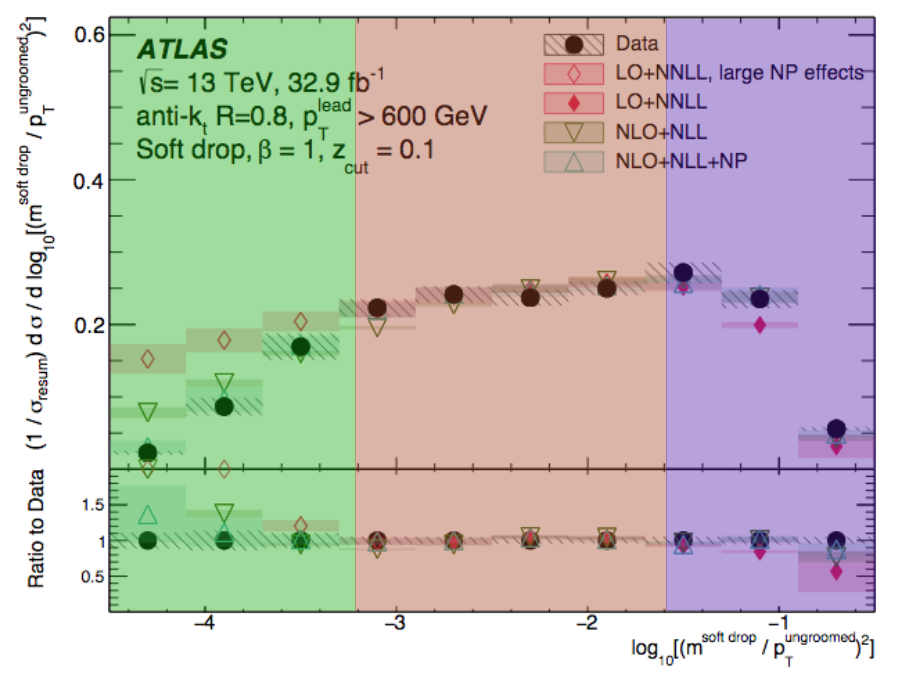
\includegraphics[width=.60\textwidth]{visuals/ATLAS-rho-highorder.png}
\caption{Above is the ATLAS Dijets dimensionless mass result ~\cite{Dreyer:2018nbf}.Next to Leading Order + Next to Leading Log + NonPerturbative corrections were required in order to match data in non-perturbative regime (Far left of this plot, shaded green column).}
\label{fig:atlasDijet}
\end{figure}




%%%%%%%%%%%%%%%%%%%%%%%%%%%%%%%%%%%%%%%%%%%%%%%%%%%%%%%%%%%%%%%%%%%%%%%%%%%%%%


\subsection{Initial-State Radiation Contributions to Jet Mass }\label{sec:jetmassISR}


To expand upon the simple calculation above to include additional emissions, one can consider the case of emission of a soft gluon from a dipole formed by 2 hard quarks. This process is illustrated in Figure ~\ref{softgluon}.



\begin{figure}[htb]
\centering
\includegraphics[width=.60\textwidth]{visuals/softgluon.png}
\caption{Above the incoming hard partons, of momenta $p_1$ and $p_2$, form a jet of momentum $p_3$ and a soft gluon of momentum $k_t$ is radiated as initial state radiation. For simplicity the assumption is made that the jet was produced at $\phi = 0$  }
\label{softgluon}
\end{figure}


If the soft gluon from the kinematic diagram is clustered with the jet then it will make the following contribution to the jet mass ~\cite{Marzani:2019hun}:\newline


\begin{equation}
m^{2}=\left(p_{3}+k\right)^{2}=2 p_{3} \cdot k=2 p_{t} k_{t}(\cosh (\eta-y)-\cos \phi)
\end{equation}

Given the above, one can write the contribution to the cumulative distribution as :\newline

\begin{equation}
\begin{aligned} \alpha_{s} \Sigma_{12}^{(1)} &=C_{12} \int k_{t} d k_{t} d \eta \frac{d \phi}{2 \pi} \frac{\alpha_{s}\left(\kappa_{12}\right)}{2 \pi} \frac{\left(p_{1} \cdot p_{2}\right)}{\left(p_{1} \cdot k\right)\left(p_{2} \cdot k\right)} \Theta\left((\eta-y)^{2}+\phi^{2}<R^{2}\right) \\ & \cdot\left(\frac{2 k_{t}}{p_{t} R^{2}}(\cosh (\eta-y)-\cos \phi)>\rho\right) \end{aligned}
\end{equation}

$\Theta$ is the jet clustering condition~\cite{Marzani:2019hun}. Integrating and simplifying one finds:\newline

\begin{equation}
\alpha_{s} \Sigma_{12}^{(1)}=C_{12} R^{2} \int_{\rho p_{t}}^{p_{t}} \frac{\alpha_{s}\left(k_{t}\right)}{2 \pi} \frac{d k_{t}}{k_{t}}
\end{equation}

The equation tells us that the soft gluon will not give rise to collinear enhancements since it is away from the hard partons in the process. The lower limit on the integration comes from the jet mass constraint.

%%%%%%%%%%%%%%%%%%%%%%%%%%%%%%%%%%%%%%%%%%%%%%%%%%%%%%%%%%%%%%%%%%%%%%%%%%%%%%%



%%%%%%%%%%%%%%%%%%%%%%%%%%%%%%%%%%%%%%%%%%%%%%%%%%%%%%%%%%%%%%%%%%%%%%%%%%%%%%


\subsection{Jet Mass in Proton-Proton $\rightarrow$ Z + jet }\label{sec:jetmass}

The specific jet production channel studied in this thesis is Z + jet. This process is useful to study as it produces a sample of light quark enriched jets for the measurement as opposed to the dijet measurements previously performed by CMS and ATLAS, those studied a quark-gluon admixture enriched jet sample. In principle, the interaction is simpler than the dijet case having only 3 coloured hard legs as opposed to 4~\cite{Marzani:2019hun}. Additionally, the Z + jets channel is interesting to understand in the boosted regime, $\pt >> m$ , as it is the main background in searches for a boosted Higgs boson recoiling off a Z boson ~\cite{Marzani:2019hun}.





The Figure ~\ref{fig:quarkandgluoninzplusjet}, shows calculations at Born level for 2 partonic processes: $q g \rightarrow Z q$ and $q \bar{q} \rightarrow Z g $ . The Feynman diagrams for these processes are shown on the bottom and top respectively, of Figure ~\ref{fig:feynmanzjet}.

\begin{figure}[htb]
\centering
\includegraphics[width=.60\textwidth]{visuals/feynmanZjet.png}
\caption{The LO Feynman diagrams for (Top) The Compton Process (Bottom) Quark - Anti-Quark Annihilation, the top being far more likely to occur at LHC. }
\label{fig:feynmanZjet}
\end{figure}


In Figure ~\ref{fig:quarkandgluoninzplusjet} it is noteworthy to realize that the bulk of the order $R^2$ corrections (black line) are composed of contributions from the simple ISR gluon as illustrated in Section ~\ref{sec:jetmassISR}



\subsection{Groomed Jet Mass }\label{sec:jetmassgroomed}

The jet mass distribution for soft-dropped jets differs from the plain jet because it lacks soft and collinear radiation contributions. It is shown in the Lund diagram in Figure ~\ref{fig:mmdtsoftdropLund} at LL accuracy, where the shaded red area is that vetoed and associated with Sudakov suppression and the red line is a line of constant jet $\rho$.

\begin{figure}[htb]
\centering
\includegraphics[width=.60\textwidth]{visuals/mmdtsoftdropLund.png}
\caption{Lund diagrams for : (a) The modified mass drop tagger, (b) The Soft-Drop procedure . The dotted green line is the edge of the dropped region in both cases. }
\label{fig:mmdtsoftdropLund}
\end{figure}

For the soft-dropped mass the LO cumulative distribution can be written as :\newline

\begin{equation}
\begin{aligned} \Sigma_{\mathrm{SD}}^{(\mathrm{LO})}(\rho) &=\frac{1}{\sigma_{0}} \int_{0}^{\rho} d \rho^{\prime} \frac{d \sigma}{d \rho^{\prime}}=1-\frac{1}{\sigma_{0}} \int_{\rho}^{1} d \rho^{\prime} \frac{d \sigma}{d \rho^{\prime}} & & \\ &\left(1-\frac{\alpha_{s} C_{F}}{\pi}\left[\frac{1}{2} \log ^{2}\left(\frac{1}{\rho}\right)-\frac{3}{4} \log \left(\frac{1}{\rho}\right)\right],\right.& \text { if } \quad \rho>z_{\mathrm{cut}} \\ 1-\frac{\alpha_{s} C_{F}}{\pi} &\left[\frac{1}{2} \log ^{2}\left(\frac{1}{\rho}\right)-\frac{1}{2+\beta} \log ^{2}\left(\frac{z_{\text {cut }}}{\rho}\right)-\frac{3}{4} \log \left(\frac{1}{\rho}\right)\right], & \text { if } \quad \rho<z_{\text {cut }} \end{aligned}
\end{equation}

at order $\alpha_s$~\cite{Marzani:2019hun}.

Since many of the complications of the calculations, such as non-global logarithms, are eliminated by dropping the soft and collinear contributions theorists are able to analytically calculate the soft-drop groomed jet mass and perform an all-order resummation of the logarithms.

\begin{equation}
\Sigma_{\mathrm{SD}}(\rho)=\exp \left[-R_{\mathrm{SD}}(\rho)\right]
\end{equation}



\begin{equation}
R_{\mathrm{SD}}(\rho)=\int_{0}^{1} \frac{d \theta^{2}}{\theta^{2}} d z P_{i}(z) \frac{\alpha_{s}\left(z \theta p_{t} R\right)}{2 \pi} \Theta\left(z \theta^{2}>\rho\right) \Theta\left(z>z_{\mathrm{cut}} \theta^{\beta}\right)
\end{equation}


Including the following term accounts for a running coupling correction~\cite{Marzani:2019hun}

\begin{equation}
\alpha_{s}\left(z \theta p_{t} R\right)=\frac{\alpha_{s}\left(p_{t} R\right)}{1+2 \alpha_{s} \beta_{0} \log (z \theta)}
\end{equation}


Performing the integration retaining only hard-collinear branchings, Equation ~\ref{hard}, and only the leading double-logarithm contributions from soft and collinear emissions~\cite{Marzani:2019hun}, Equation ~\ref{soft}.



\begin{equation}
R_{\mathrm{SD}}^{(\mathrm{LL})}(\rho)=\frac{C_{i}}{2 \pi \alpha_{s} \beta_{0}^{2}}\left[\frac{2+\beta}{1+\beta} W\left(1-\frac{\lambda_{c}+(1+\beta) \lambda_{\rho}}{2+\beta}\right)-\frac{W\left(1-\lambda_{c}\right)}{1+\beta}-2 W\left(1-\frac{\lambda_{\rho}}{2}\right)\right.
\end{equation}\label{soft}



\begin{equation}
\left.-2 \alpha_{s} \beta_{0} B_{i} \log \left(1-\frac{\lambda_{\rho}}{2}\right)\right]
\end{equation}\label{hard}

where

\begin{equation}
\lambda_{\rho}=2 \alpha_{s} \beta_{0} \log (1 / \rho), \quad \lambda_{c}=2 \alpha_{s} \beta_{0} \log \left(1 / z_{\mathrm{cut}}\right), \quad \text { and } \quad W(x)=x \log (x)
\end{equation}



Lastly, the expression can be expanded up to NNLL corrections~\cite{Marzani:2019hun}:

\begin{equation}
R_{\mathrm{SD}}^{(\mathrm{LL})}(\rho)=\frac{C_{i}}{2 \pi \alpha_{s} \beta_{0}^{2}}\left[\frac{2+\beta}{1+\beta} W\left(1-\frac{\lambda_{c}+(1+\beta) \lambda_{\rho}}{2+\beta}\right)-\frac{W\left(1-\lambda_{c}\right)}{1+\beta}-2 W\left(1-\frac{\lambda_{\rho}+\lambda_{B}}{2}\right)\right.
\end{equation}


\begin{equation}
\left.+W\left(1-\lambda_{B}\right)\right]
\end{equation}

Define 
\begin{equation}
\lambda_{B}=-2 \alpha_{s} \beta_{0} B_{i}
\end{equation}.



% pilup images with diff algorithms
%# https://arxiv.org/pdf/1304.1025.pdf
%Sequential recombination algorithm for jet clustering and

%Towards Jetography
%Gavin P. Salam
%$https://arxiv.org/abs/0906.1833
%\cite{Salam:2009jx}

%\cite{Asquith:2018igt}
%https://arxiv.org/pdf/1803.06991.pdf
%Jet Substructure at the Large HadronCollider :  Experimental Review

%%%%%%%%%%%%%%%%%%%%%%%%%%%%%%%%%%%%%%%%%%%%%%%%%%%%%%%%%%%%%%%%%%%%%%%%%%%%%%%%%%%%%%%%%

% DY thesis https://cds.cern.ch/record/2018454/files/CERN-THESIS-2015-048.pdf
